\documentclass{beamer}

\mode<presentation> {

%\usetheme{default}
%\usetheme{AnnArbor}
%\usetheme{Antibes}
%\usetheme{Bergen}
%\usetheme{Berkeley}
%\usetheme{Berlin}
%\usetheme{Boadilla}
%\usetheme{CambridgeUS}
%\usetheme{Copenhagen}
%\usetheme{Darmstadt}
% \usetheme{Dresden}
%\usetheme{Frankfurt}
%\usetheme{Goettingen}
%\usetheme{Hannover}
%\usetheme{Ilmenau}
%\usetheme{JuanLesPins}
%\usetheme{Luebeck}
\usetheme{Madrid}
%\usetheme{Malmoe}
%\usetheme{Marburg}
%\usetheme{Montpellier}
%\usetheme{PaloAlto}
%\usetheme{Pittsburgh}
%\usetheme{Rochester}
%\usetheme{Singapore}
%\usetheme{Szeged}
%\usetheme{Warsaw}


%\usecolortheme{albatross}
%\usecolortheme{beaver}
%\usecolortheme{beetle}
%\usecolortheme{crane}
%\usecolortheme{dolphin}
%\usecolortheme{dove}
%\usecolortheme{fly}
%\usecolortheme{lily}
%\usecolortheme{orchid}
%\usecolortheme{rose}
%\usecolortheme{seagull}
%\usecolortheme{seahorse}
%\usecolortheme{whale}
%\usecolortheme{wolverine}

%\setbeamertemplate{footline} % To remove the footer line in all slides uncomment this line
%\setbeamertemplate{footline}[page number] % To replace the footer line in all slides with a simple slide count uncomment this line

%\setbeamertemplate{navigation symbols}{} % To remove the navigation symbols from the bottom of all slides uncomment this line
}

\usepackage{graphicx} % Allows including images
\usepackage{booktabs} % Allows the use of \toprule, \midrule and \bottomrule in tables
\usepackage{amsfonts}
\usepackage{mathrsfs, bbold}
\usepackage{amsmath,amssymb,graphicx}
\usepackage{mathtools} % gather
\usepackage[export]{adjustbox} % right-aligned graphics

% tikz?
\usepackage{tikz}
\usetikzlibrary{arrows, shapes}


\usepackage[style=authortitle,backend=bibtex]{biblatex}
%\usepackage[backend=biber,style=numeric-comp,sorting=none]{biblatex}
\addbibresource{references.bib}

%----------------------------------------------------------------------------------------
%	TITLE PAGE
%----------------------------------------------------------------------------------------

\title["10"]{10: Introduction to Bayesian Computation}

% \author{Taylor} 
% \institute[UVA] 
% {
% University of Virginia \\
% \medskip
% \textit{} 
% }
\date{10/30/19} 
    
\begin{document}
%----------------------------------------------------------------------------------------

\begin{frame}
\titlepage 
\end{frame}

%----------------------------------------------------------------------------------------


\begin{frame}
\tableofcontents
\end{frame}


%----------------------------------------------------------------------------------------
\section{Importance Sampling with Resampling}
\begin{frame}[fragile]
\frametitle{Adding Resampling}

Importance Sampling gives you weighted draws $(\theta^1, w(\theta^1) ), (\theta^2, w(\theta^2) ), \ldots$
\newline

You can draw from these, with replacement. At the expense of more variance, it will give you unweighted draws from your target distribution:
$\tilde{\theta}^1, \tilde{\theta}^2, \ldots $
\newline

This is known as {\bf factored sampling} or {\bf importance sampling with resampling} or {\bf sampling importance resampling} (SIR).


\end{frame}

%----------------------------------------------------------------------------------------
\begin{frame}[fragile]
\frametitle{Adding Resampling}

\begin{center}
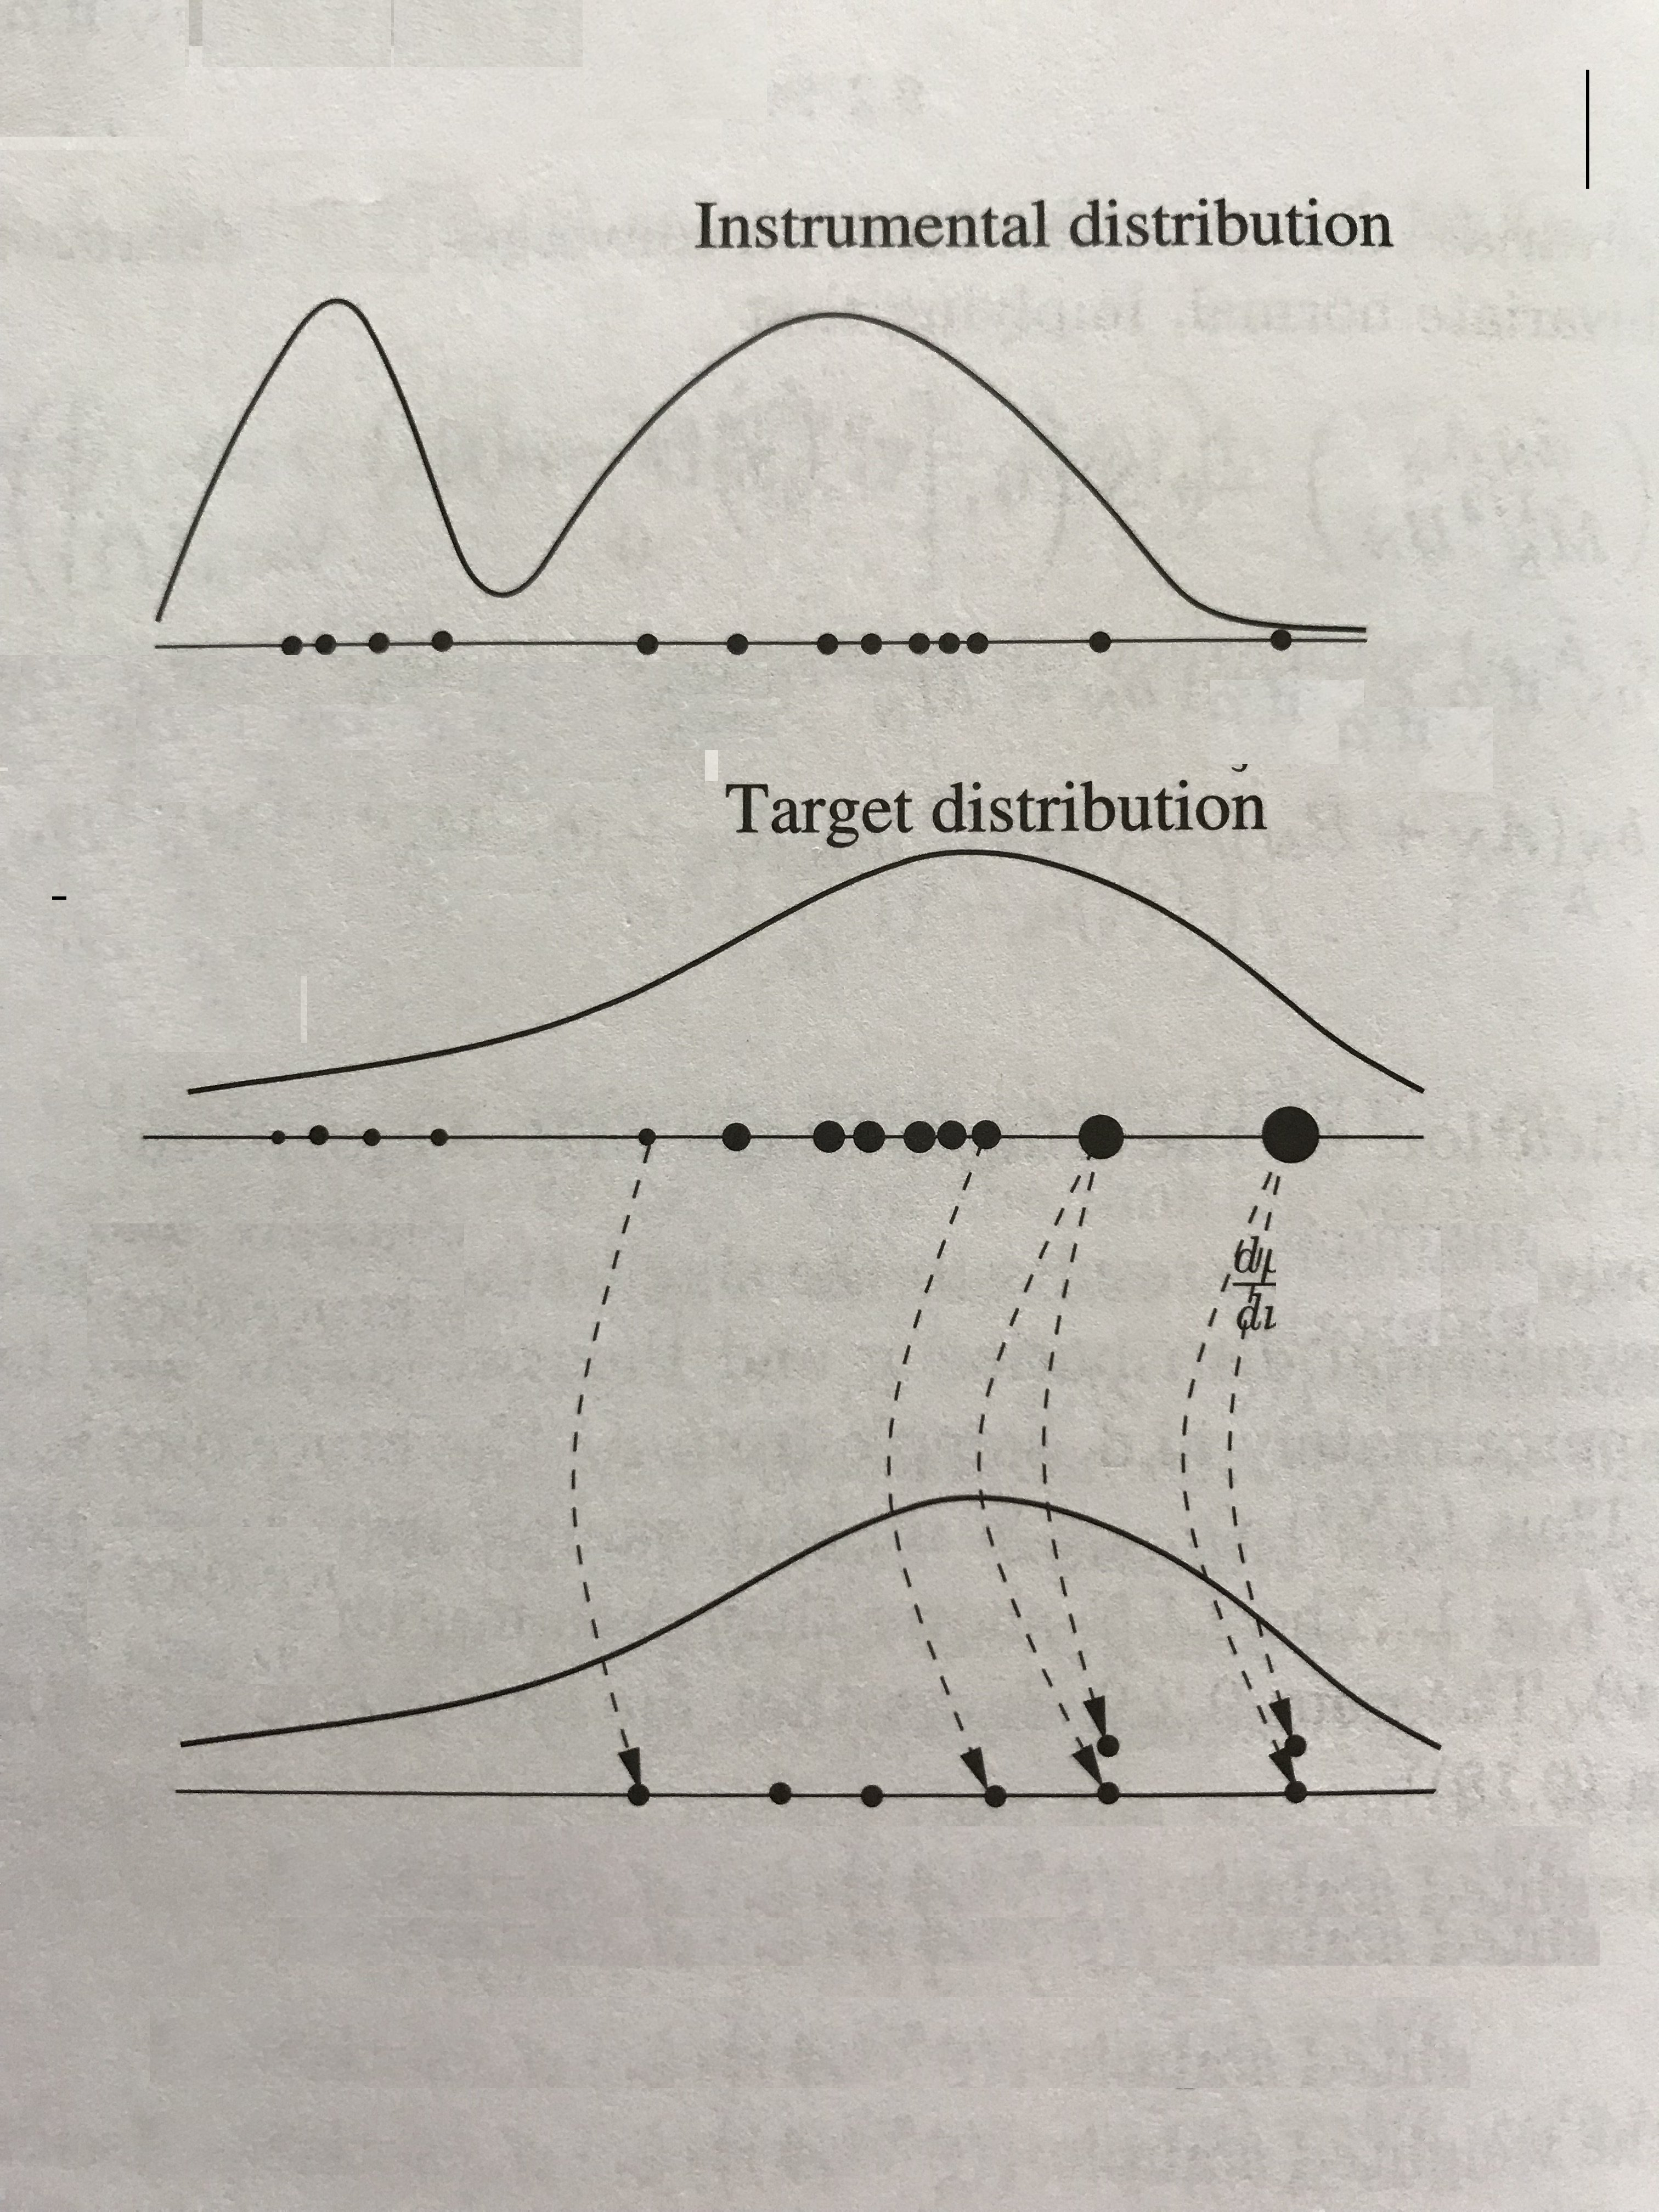
\includegraphics[width=50mm]{isr.jpg}
\end{center}
Original, unedited image is from \url{https://www.springer.com/us/book/9780387402642}

\end{frame}




% homework question: https://stats.stackexchange.com/questions/359977/conditional-expectation-on-an-estimator-for-defensive-sampling

%----------------------------------------------------------------------------------------
\begin{frame}[fragile]
\frametitle{SIR}


Stage 1: do importance sampling to get $\{ \theta^i, w(\theta^i) \}_{i=1}^S$.
\newline

Stage 2: for $i = 1, \ldots, S$, select 
$$
P[ \tilde{\theta}^i = \theta^j \mid \theta^1, w(\theta^1), \ldots,
\theta^S, w(\theta^S) ] = w(\theta^j).
$$

\end{frame}

% %----------------------------------------------------------------------------------------
% \begin{frame}[fragile]
% \frametitle{SIR}

% Another way to write it:
% \newline

% Stage 1: do importance sampling to get $\{ \theta^i, w(\theta^i) \}_{i=1}^S$.
% \newline

% Stage 2: for $i = 1, \ldots, S$, select indexes
% $$
% P[ I^i = j \mid \theta^1, w(\theta^1), \ldots, \theta^S, w(\theta^S) ] = \frac{w(\theta^j)}{ \sum_k w(\theta^k) }
% $$
% and then set 
% $$
% \tilde{\theta}^i = \theta^{I^i}.
% $$

% \end{frame}


%----------------------------------------------------------------------------------------
\begin{frame}[fragile]
\frametitle{Example 2 revisited}

\begin{verbatim}
y <- 2 # fake data
log_unnorm_weight <- function(theta){ 
  # can ignore sqrt(2pi) because it will cancel out
  -.5*(y - theta)^2 }
num_samples <- 10000
theta_draws <- rt(num_samples , 1)
lunws <- log_unnorm_weight(theta_draws)
# note: prob arg automatically normalizes
random_indexes <- sample(x = num_samples, 
                         size = num_samples, 
                         replace = T, 
                         prob = exp(lunws)) 
sort(random_indexes) # see there are repeats!
resampled_draws <- theta_draws[random_indexes]
hist(resampled_draws) # can't do this unless we resample
\end{verbatim}

\end{frame}


%----------------------------------------------------------------------------------------
\begin{frame}[fragile]
  \frametitle{Other uses of importance (re)sampling}
  \begin{itemize}
  \item Use importance resampling for obtaining starting points for an
    iterative simulation of the posterior distribution, as in Chapter
    11.
\pause
\item Calculation of intractable quantity under a change of model.\\

Posterior under the previous model: $p_1(\theta|y) \propto q_1(\theta|y)$

$\theta^1, \ldots, \theta^S \sim p_1(\theta|y)$

Posterior after a change of model: $p_2(\theta|y) \propto q_2(\theta|y)$

We need $E_2(h(\theta)|y)$
\pause

Importance sampling with $g(\theta) = q_1(\theta|y)$,
$\tilde{w}(\theta) = q_2(\theta|y)/q_1(\theta|y)$, $w(\theta^s) =
\tilde{w}(\theta^s)/\sum_{l=1}^S \tilde{w}(\theta^l)$
\[
E_2(h(\theta)|y) = \sum_{i=1}^S h(\theta^s) w(\theta^s)
\]
\end{itemize}
\end{frame}


%----------------------------------------------------------------------------------------
\section{Sequential Monte Carlo}
\begin{frame}[fragile]
\frametitle{Going sequential}

Resampling adds variance, so why do it?
\newline

It throws away bad samples, and duplicates promising ones. 
\newline

When you're looking at a sequence of distribution targets, this can have a good effect on future samples.
\pause
\newline

{\bf sequential monte carlo} or {\bf particle filtering} methods are basically doing SIR over and over again. 
\newline

At ``time" $t-1$ you just resampled, so you have draws $\tilde{\theta}^1_{t-1}, \tilde{\theta}^2_{t-1}, \ldots, \tilde{\theta}^S_{t-1}$, and you want to turn them into draws for the next ``time" period:
$$
\tilde{\theta}^1_{t}, \tilde{\theta}^2_{t}, \ldots, \tilde{\theta}^S_{t}.
$$

\end{frame}

%----------------------------------------------------------------------------------------
\begin{frame}[fragile]
\frametitle{Examples of sequences of distributions}

{\bf Data annealing} \footcite{Chopin}
\[
p(\theta), p(\theta \mid y_1), p(\theta \mid y_{1:2}), \ldots, p(\theta \mid y_{1:n}),
\]

{\bf Temperature annealing} \footcite{Neal}
\[
p(y \mid \theta)^{a_0} p(\theta), p(y \mid \theta)^{a_1} p(\theta),  \ldots p(y \mid \theta)^{a_n} p(\theta)
\]
with $0 = a_0 < a_1 < \cdots < a_n = 1$. 
\newline


{\bf filtering and smoothing} in state space models
\[
p(x_1 \mid y_1, \theta), \ldots , p(x_{n} \mid y_{1:n}, \theta)
\]

\end{frame}

%----------------------------------------------------------------------------------------
\begin{frame}[fragile]
\frametitle{state space models}

\tikzstyle{format} = [draw, thin, fill=blue!20]
\tikzstyle{medium} = [ellipse, draw, thin, fill=green!20, minimum height=2.5em]

\begin{figure}
\begin{tikzpicture}[node distance=3cm, auto,>=latex', thick]
    % We need to set at bounding box first. Otherwise the diagram
    % will change position for each frame.
    \path[use as bounding box] (-1,0) rectangle (10,-2);
    \path[->] node (past) { $\cdots$ };
    \path[->] node[format, right of=past] (xtm1) {$x_{t-1}$}
                  (past) edge node {$f_{t-1}$} (xtm1);
    \path[->] node[format, right of=xtm1] (xt) {$x_t$}
                  node[medium, below of=xtm1] (ytm1) { $Y_{t-1}$ }
                  (xtm1) edge node { $f_{t}$ } (xt)
                        edge node[swap] { $g_{t-1}$ } (ytm1);
    \path[->] node[right of=xt] (future) {$\cdots$}
                  node[medium, below of=xt] (yt) {$y_t$}
                  (xt) edge node {$f_{t+1}$} (future)
                       edge node[swap] {$g_{t}$} (yt);
\end{tikzpicture}
\end{figure}
% \vspace*{\baselineskip}
% \vspace*{\baselineskip}


\begin{align*}
&p(x_{1:T}, y_{1:T} \mid \theta) \\
&= g(y_1 \mid x_1, \theta) f(x_1 \mid \theta) \prod_{t=2}^T g(y_t \mid x_t, \theta) f(x_t \mid x_{t-1}, \theta)
\end{align*}

\end{frame}
%----------------------------------------------------------------------------------------
\begin{frame}[fragile]
\frametitle{Example: filtering in state space models}

Here's an example of a state space model. $y_t$ is a univariate time series, and $x_t$ is a hidden/unobserved/latent time series.
\newline

\begin{gather}
y_t = \exp(x_t / 2) \epsilon_t \\
x_t = c + \phi x_{t-1} + v_t
\end{gather}

We sometimes refer to (1) as $g(y_t \mid x_t, \theta)$ or the observation equation, and (2) as the state transition equation or $f(x_t \mid x_{t-1}, \theta)$.
\end{frame}

%----------------------------------------------------------------------------------------
\begin{frame}[fragile]
\frametitle{Example: filtering in state space models}

$y_{1:t}$ observed, $x_{1:t}$ hidden. Goal: $p(x_t \mid y_{1:t})$ in real-time.
\newline

\begin{center}
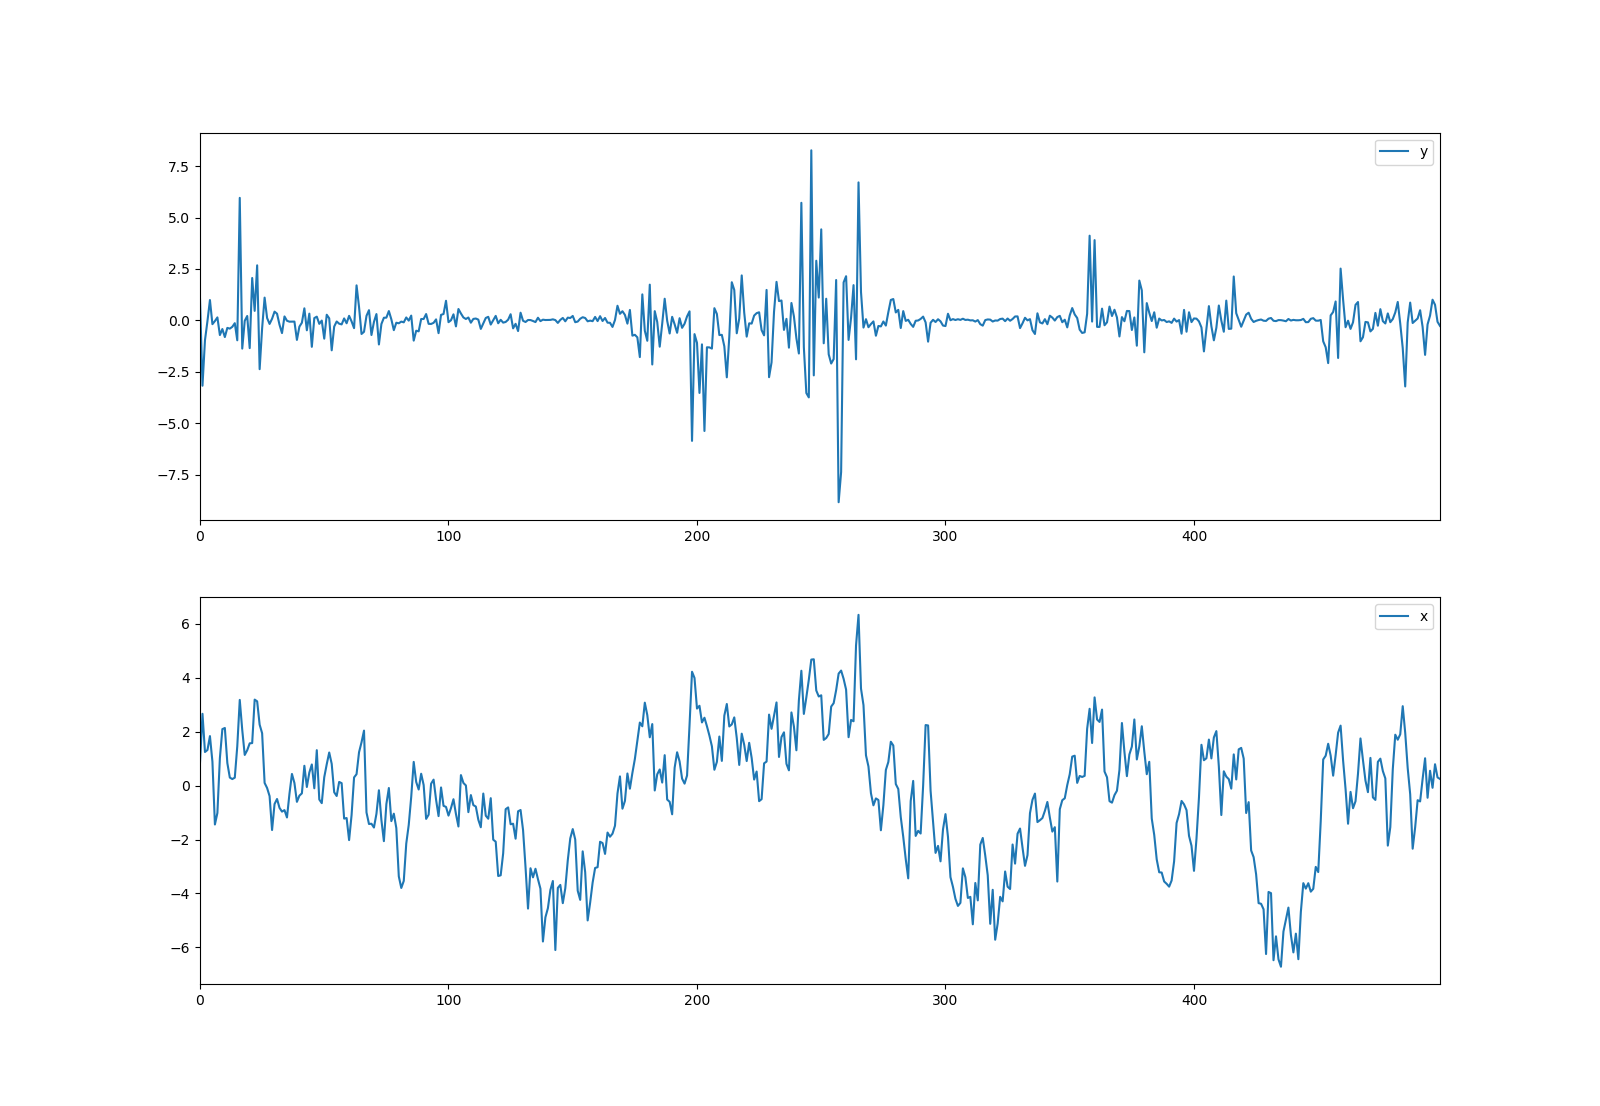
\includegraphics[width=103mm]{univ_svol_sim.png}
\end{center}

\end{frame}

%----------------------------------------------------------------------------------------
\begin{frame}[fragile]
\frametitle{Example: filtering in state space models}

\begin{center}
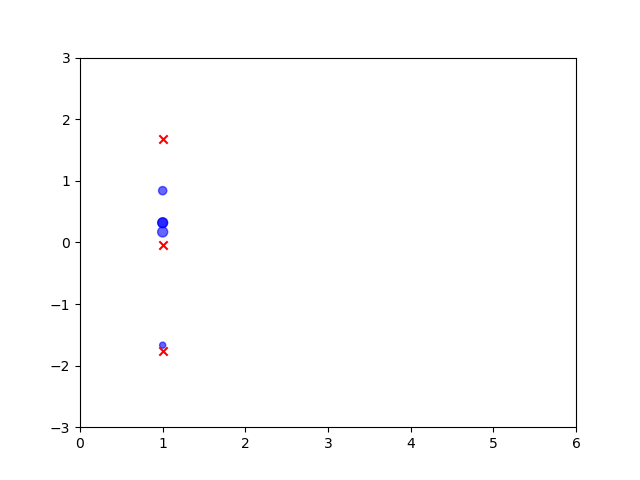
\includegraphics[width=80mm]{pfilt_anim_1.png}
\end{center}

\end{frame}

%----------------------------------------------------------------------------------------
\begin{frame}[fragile]
\frametitle{Going sequential}

\begin{center}
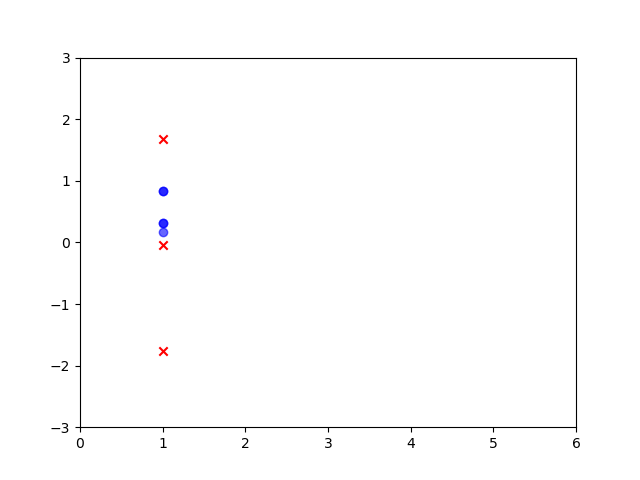
\includegraphics[width=80mm]{pfilt_anim_2.png}
\end{center}

\end{frame}

%----------------------------------------------------------------------------------------
\begin{frame}[fragile]
\frametitle{Going sequential}

\begin{center}
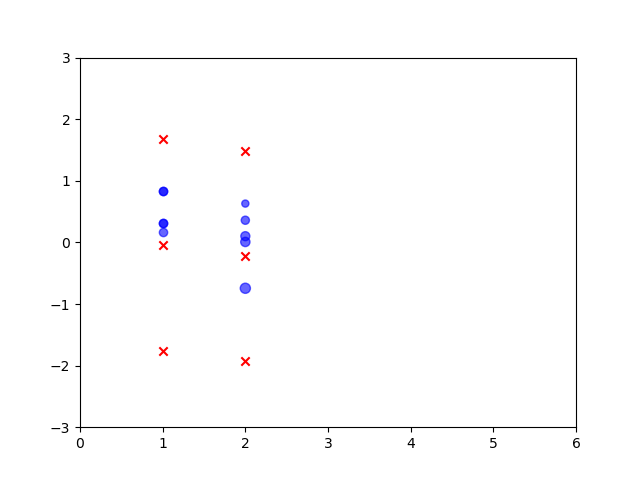
\includegraphics[width=80mm]{pfilt_anim_3.png}
\end{center}

\end{frame}
%----------------------------------------------------------------------------------------
\begin{frame}[fragile]
\frametitle{Going sequential}

\begin{center}
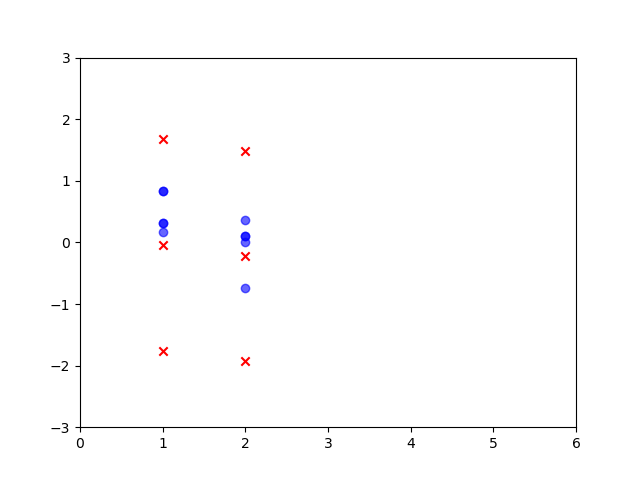
\includegraphics[width=80mm]{pfilt_anim_4.png}
\end{center}

\end{frame}
%----------------------------------------------------------------------------------------
\begin{frame}[fragile]
\frametitle{Going sequential}

\begin{center}
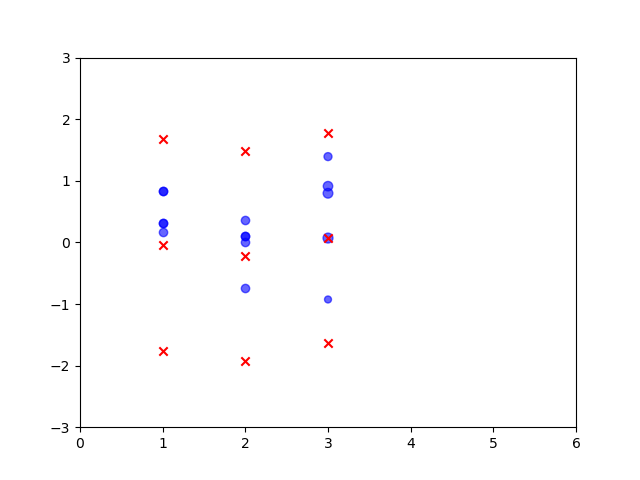
\includegraphics[width=80mm]{pfilt_anim_5.png}
\end{center}

\end{frame}
%----------------------------------------------------------------------------------------
\begin{frame}[fragile]
\frametitle{Going sequential}

\begin{center}
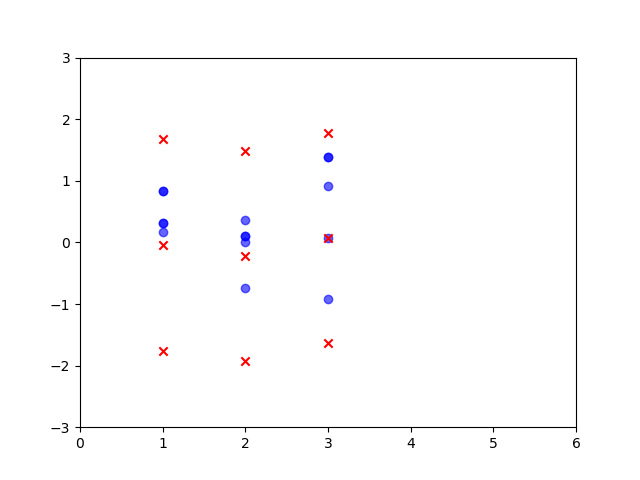
\includegraphics[width=80mm]{pfilt_anim_6.png}
\end{center}

\end{frame}
%----------------------------------------------------------------------------------------
\begin{frame}[fragile]
\frametitle{Going sequential}

\begin{center}
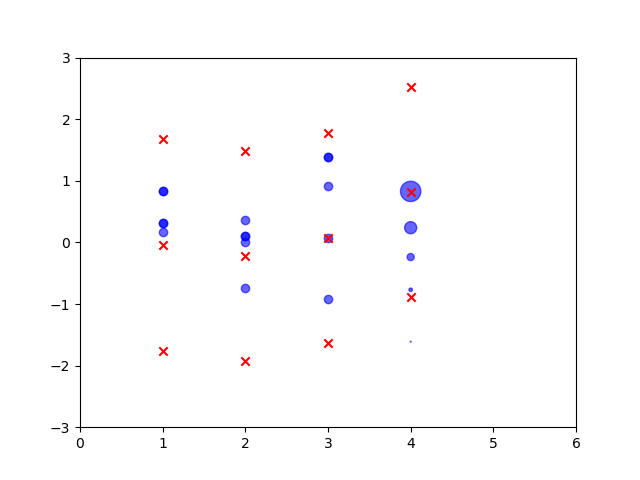
\includegraphics[width=80mm]{pfilt_anim_7.png}
\end{center}

\end{frame}
%----------------------------------------------------------------------------------------
\begin{frame}[fragile]
\frametitle{Going sequential}

\begin{center}
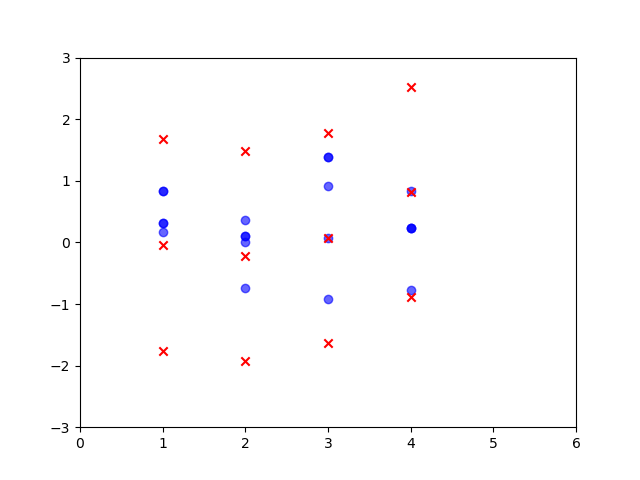
\includegraphics[width=80mm]{pfilt_anim_8.png}
\end{center}

\end{frame}
%----------------------------------------------------------------------------------------
\begin{frame}[fragile]
\frametitle{Going sequential}

\begin{center}
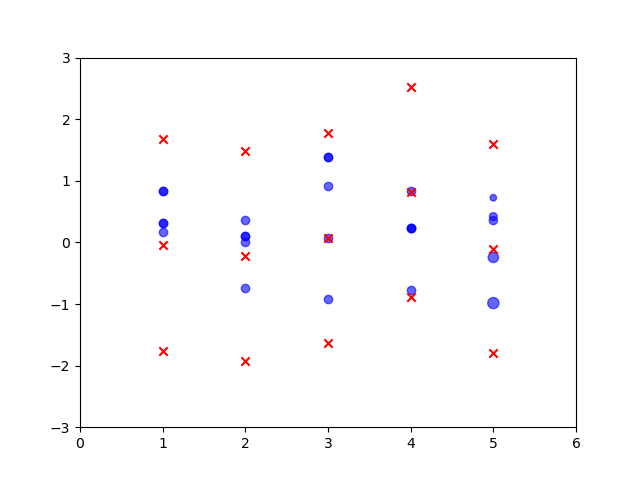
\includegraphics[width=80mm]{pfilt_anim_9.png}
\end{center}

\end{frame}
%----------------------------------------------------------------------------------------
\begin{frame}[fragile]
\frametitle{Going sequential}

\begin{center}
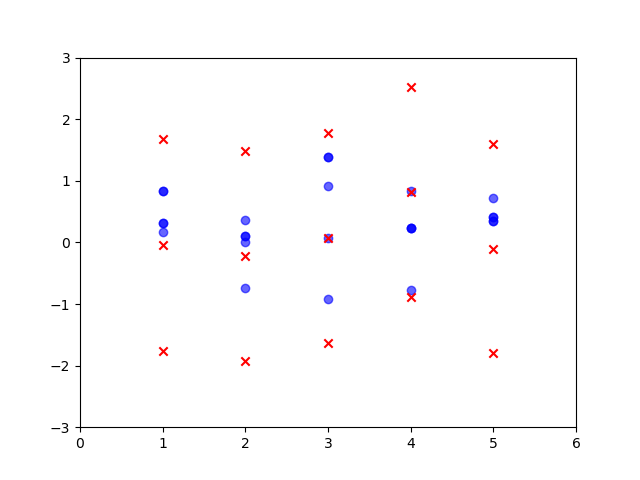
\includegraphics[width=80mm]{pfilt_anim_10.png}
\end{center}

\end{frame}




%----------------------------------------------------------------------------------------
\begin{frame}[fragile]
\frametitle{Filtering recursions}

Drop dependence on $\theta$ from the notation...
\begin{align*}
p(x_{1:t}|y_{1:t}) &=C_{t}^{-1} p(x_{t} , y_t  \mid x_{t-1})p(x_{1:t-1} \mid y_{1:t-1}) \\
&= C_{t}^{-1} \frac{p(x_t, y_t \mid x_{t-1})}{q_{t}(x_{t} \mid y_{t},x_{t-1})} \times \\
& \hspace{20mm} q_{t}(x_{t} \mid y_{t},x_{t-1})p(x_{1:t-1} \mid y_{1:t-1}) \\
&= C_{t}^{-1} \begingroup\color{red} \frac{g(y_t|x_t)f(x_t|x_{t-1})}{q_t(x_t|x_{t-1},y_t) } \endgroup \times \\
& \hspace{19mm} \begingroup\color{blue} q_t(x_t \mid x_{t-1},y_t) p(x_{1:t-1} \mid y_{1:t-1}) \endgroup\\
\end{align*}

Repeat through time:
\begin{enumerate}
\item start with samples from $p(x_{1:t-1} \mid y_{1:t-1})$
\item mutate/propogate/extend using $q_t(x_t \mid x_{t-1},y_t)$
\item adjust weights by multiplying by $ \begingroup\color{red} \frac{g(y_t|x_t)f(x_t|x_{t-1})}{q_t(x_t|x_{t-1},y_t) } \endgroup $
\item resample, giving you particles distributed as $p(x_{1:t} \mid y_{1:t})$
\end{enumerate}


\end{frame}


%----------------------------------------------------------------------------------------

\begin{frame}
\printbibliography
\end{frame}

\end{document} 




%%% Local Variables:
%%% mode: latex
%%% TeX-master: t
%%% End:
